
\chapter{Reconocimiento de Actividades}
\label{chap:Reconocimiento de Actividades}

%##Capítulo 2. Reconocimiento de Actividades
%* Introducción
%* Estructuras de datos de los Sistemas de Información Geográfica
%\input{capitulo-2/definicion-sig.tex}

\section{Introducción}
El conocimiento del contexto de usuario es una de las nuevas aplicaciones y servicios móviles en el área de la computación ubicua.
En general, el contexto de usuario significa su actividad, ubicación, preferencia, su situación, emoción, etc. Con los teléfonos móviles cada vez más potentes, la mayoría de los puntos mencionados del contexto se determinan con componentes de detección integrados en los teléfonos móviles, como acelerómetro, GPS, micrófono, bluetooth, cámara, etc. En esencia, los teléfonos móviles pueden crear redes de sensores móviles que son capaces de recoger datos de los sensores sobre la vida diaria de un usuario, es decir, quien es, lo que está haciendo el usuario, donde se encuentra, ya quien esta ? 

En este trabajo, investigamos posibilidades y viabilidades de tener un servicio para obtener el contexto de la actividad física diaria de los usuarios con teléfonos móviles.

\section{Actividades Humanas}
El diseño de un sistema HAR depende totalmente de las actividades definidas que van a ser reconocida. Por lo tanto, el cambio del conjunto de actividades que el sistema reconoce convierte al problema en uno completamente diferente al anterior.

Teniendo en cuenta esto, las distintas publicaciones, tenemos estos siete distintos grupos de actividades en la siguiente tabla.

\newcommand{\rr}{\raggedright}
\newcommand{\tn}{\tabularnewline}

\begin{table}[htbp]
	\begin{center}
		\begin{tabular}{|l|p{9cm}|}
			\hline
			\textbf{Grupo} & \textbf{Actividades} \\
			\hline \hline
			Ambulatoria & Caminar, correr, sentarse, pararse, quedarse quieto, acostarse, subir escaleras, descender escaleras, usar escaleras mecánicas, usar elevador.\\ \hline
			Transporte & Andar en bus, bicicleta y conducir \\ \hline
			En el teléfono & Enviar mensajes de texto y hacer llamadas \\ \hline
			Actividades diarias & Comer, beber, trabajar en la PC, mirar TV, leer, cepillarse los dientes, aspirar el piso, y otros. \\ \hline
			Ejercitarse & Alzar pesas, bicicleta estática, remo y otros. \\ \hline
			Militares & Arrastrarse, en cuclillas, abrir la puerta \\ \hline
			Parte superior del cuerpo & Masticar, hablar, mover la cabeza, tragar líquidos, mirar. \\ \hline
		\end{tabular}
		\caption{Grupos de Actividades.}
		\label{tabla:sencilla}
	\end{center}
\end{table}


\section{Dispositivos Móviles}
Los dispositivos móviles, tales como teléfonos móviles, reproductores de música o relojes inteligentes, han comenzado ya hace un par de años incorporar un diversos sensores. Algunos de los sensores son GPS, de audio (micrófonos), de imágenes (cámaras), de luz, sensores de temperatura, sensor de dirección (brújula), y acelerómetro.
Debido a su tamaño reducido de estos dispositivos inteligentes, su enorme capacidad de procesamiento, la posibilidad de recibir y enviar datos; y su omnipresencia en nuestra sociedad de hoy, lo hacen dispositivos de preferencia para utilizarlo en la implementación de un sistema reconocedor de actividades Humanas.

\section{Sensores ambientales vs Sensores <<Wearables>>}

En la problemática del reconocimiento de la actividad que esta realizando una persona uno de los puntos importantes a considerar es la elección de los sensores a utilizar. Los sensores pueden medir signos vitales (ritmo cardíaco, temperatura del cuerpo, presión arterial), el ambiente (intensidad de luz, temperatura, niveles de sonido), movimiento (aceleración, velocidad), y posición (localización global o en interiores).
Sobre la localización de los sensores respecto a la persona, algunos autores \cite{ReyesOrtiz2015} diferencian entre ambientales, cuando los sensores esta ubicados de manera estatica en el ambiente que rodea a la persona, y <<wearables>> cuando lo sensores se usan o están conectados al cuerpo de la persona.

\subsection{Sensores Ambientales}

Los sensores ambientales, también denominados externos o de entorno, son un conjunto de dispositivos que se encuentran en el medio ambiente que miden propiedades físicas del entorno donde las personas se encuentras e interactúan. Existe una amplia variedad de sensores ambientales, como micrófonos, cámaras de vídeo, sensores de presencia, termómetros y sensores de profundidad(Kinect). Para este tipo de reconocimiento tenemos por ejemplo a \cite{Poppe2007} que realiza un análisis de movimientos humanos utilizando cámaras de vídeo.

\subsection{Sensores <<Wearables>>}

Los sensores <<Wearables>> son usados para obtener señales directamente en una persona, estos pueden estar unidos a varias partes del cuerpo, como ser la cintura, muñeca, pecho, pierna, y cabeza(agregar referencia un paper con dispositivo en brazo/pierna/etc) pero también pueden formar parte de la ropa o embebido en otro accesorio de uso común, como relojes, anteojos, o teléfonos móviles. Como característica tienen una batería que proporciona la energía para poder operar, y algunos cuentan con conexión inalámbrica wifi/bluetooh para la transmisión de los datos obtenidos.

Señales del movimientos y físicas son obtenidas por los sensores, como ser temperatura de la piel, frecuencia cardíaca, conductividad, y posicionamiento global (GPS), posicionamiento en interiores y movimientos del cuerpo. Todos estas mediciones son utilices para tener una constante información del estado de una persona en cualquier momento.

Después hay que mencionar que dentro de los wearables están los que usan sensores acelerómetro en varias partes del cuerpo y los que usan acelerómetro de teléfonos moviles.

Otros autores como \cite{karmul2010} extraen al reconocimiento con cámaras de vídeo como una clasificación diferente a los ambientales. 


\section{Metodología HAR}
Al igual que en otras aplicaciones de aprendizaje automático, la actividad el reconocimiento requiere dos etapas, es decir, entrenamiento y las pruebas o evaluación.

\begin{figure}[!htbp]
\centering
	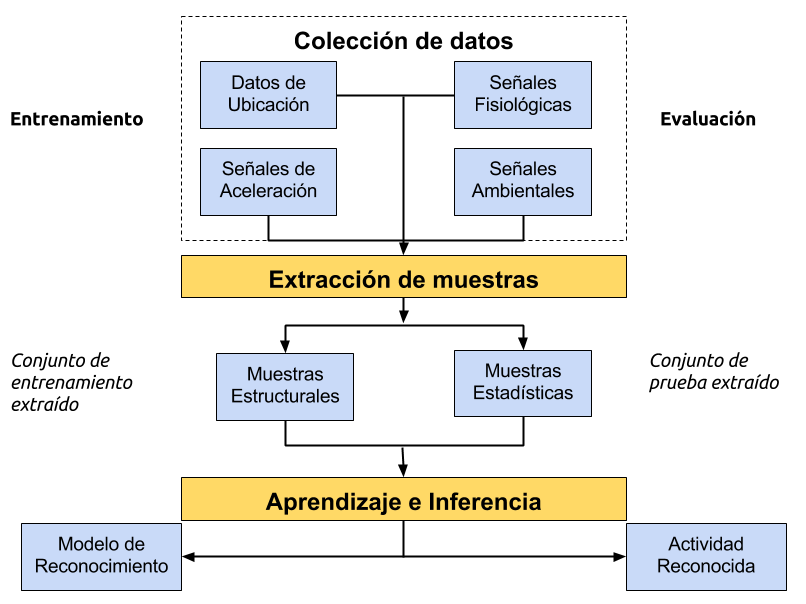
\includegraphics[width=0.7\linewidth]{capitulo-2/graphics/harsystem}
	\caption[Flujo HAR]{Flujo general del Reconocimiento de Actividades Humanas (HAR)}
	\label{fig:harsystem}
\end{figure}

En la \figref{fig:harsystem} se visualiza las fases comunes de las dos etapas. La etapa de entrenamiento requiere inicialmente un conjunto de datos recolectados en una serie de tiempo con los atributos medidos a partir de individuos que realizan cada actividad. Las series de tiempo se divide en ventanas de tiempo para aplicar la extracción de muestras filtrando así la información relevante en las señales en bruto. Más tarde, los métodos de aprendizaje se utilizan para generar un modelo de reconocimiento de actividades del conjunto de datos colectado a través de las características calculadas. Del mismo modo, para la etapa de prueba o evaluación, se recogen datos durante una ventana de tiempo, que se utiliza para extraer las mismas características utilizadas en el modelo,  estas se evalúan en el modelo de aprendizaje previamente  entrenado, generando una etiqueta de la actividad predicha.

Para cada estaba tenemos puntos a tener en cuenta:

\subsection{Colección de Datos}
La definición del método de colección de datos es un punto importante en un HAR. Según como se realiza la observación del individuo existen: ambientes realistas, que son los ideales pero no siempre es posible realizar este tipo de colectas. También existen los ambientes semirealistas que se realizan en laboratorios simulando las condiciones reales de las actividades. Por otro lado tenemos los ambientes totalmente controlados en laboratorio.

Una falla en el diseño de un sistema HAR se puede dar por no considerar las condiciones reales de las actividades, tales como actividades no tenidas en cuenta, calibración de sensores, ruido, etc.

Otra de las consideraciones a tener en cuenta en este punto es la cantidad de individuos para realizar la colección, es recomendable el mayor cantidad de individuos en distintos tipos de edades y condiciones físicas. 


\subsection{Selección y Extracción de Características}
Para cualquier problema de aprendizaje automático, la selección de características se refiere al proceso de selección de un conjunto significativo de características que aporten relevancia a la capacidad de discriminación en un algoritmo de aprendizaje. Por otro lado, la extracción de características, tiene como objetivo disminuir la cantidad de características a utilizar mediante distintas transformaciones entre ellas para obtener nuevas características reducidas sin perder información relevante del conjunto de datos originales. La selección y extracción de características también permite reducir los tiempos de procesamiento en la fase de entrenamiento y aumenta el rendimiento en la fase de evaluación 

Dependiendo de la aplicación, las características requeridas para la extracción de la información relevante pueden variar. En el caso particular de HAR, una representación reducida de los datos del sensor se puede utilizar como la entrada del algoritmo de reconocimiento. Esto se logra mediante medición de la señal del sensor en varios dominios, pudiendo ser en tiempo y frecuencia.

\subsection{Métodos de Aprendizaje}
Varios enfoques de LD se han desarrollado a lo largo de los años para HAR. En su mayoría a través de algoritmos de aprendizaje supervisado aunque también se han propuesto métodos semi-supervisados y no supervisados.

Modelos bayesianos y basados en frecuencia han sido bien cubierto en toda la literatura HAR. Implican modelos basados en reglas como Arboles de decisión y Selvas Aleatorias, algunos con un enfoques geométrico k-NN, ANN y SVM, y los métodos de clasificación probabilísticos, por ejemplo clasificadores bayesiano, y modelos ocultos de Markov (HMM).

Otros aspectos relevantes para la selección del algoritmo de modelo de aprendizaje incluyen: el consumo de energía, los requisitos de memoria, interpretabilidad y complejidad computacional, etc. Estos aspectos se agudizan si se utilizan dispositivos inteligentes .Como cuestión de ejemplo, árboles de decisión podrían ser preferidos cuando se requiere simplicidad en su implementación y SVMs para aplicaciones de alto rendimiento.

En el capitulo \ref{chap:Aprendizaje-Automatico} se detalla todo lo referente a métodos de aprendizaje y los utilizados en este trabajo.

\subsection{Definición del Problema}
Teniendo en cuenta todo esto puntos podemos definir el problema como:

\newtheorem{defi}{Definición}

\begin{defi}(HARP)
	Dado un conjunto $S = \{S_{0},...,S_{k-1}\} $ de $k$ series de tiempo, cada una medida de cada atributo, y todo definido en un intervalo de tiempo $I =  \left [ t_{\alpha}, t_{\omega} \right ]$ el objetivo es encontrar un sub intervalo de tiempo $\left\langle I_{0},...,I_{r-1} \right\rangle $ en $I$, basado en datos de $S$ y conjunto de etiquetas que representan la actividad realizada durante cada intervalo $I_{j}$ (Ej. sentado, caminando, corriendo, etc.). Esto implica que cada intervalo $I_{j}$ son consecutivos, no vacíos, no superpuestos y tal que $ \displaystyle\bigcup_{r-1}^{j=0}{I_j = I } $
\end{defi}

Note que el HARP no es factible una resolución determinista. El numero de combinaciones de valores de atributos y actividades puede ser muy grande a veces infinito; y encontrar los puntos de transición es complicado teniendo en cuenta que se desconoce la duración de las actividades.

